\documentclass[12pt,]{article}
\usepackage[left=1in,top=1in,right=1in,bottom=1in]{geometry}
\newcommand*{\authorfont}{\fontfamily{phv}\selectfont}
\usepackage{lmodern}


  \usepackage[T1]{fontenc}
  \usepackage[utf8]{inputenc}



\usepackage{abstract}
\renewcommand{\abstractname}{}    % clear the title
\renewcommand{\absnamepos}{empty} % originally center

\renewenvironment{abstract}
 {{%
    \setlength{\leftmargin}{0mm}
    \setlength{\rightmargin}{\leftmargin}%
  }%
  \relax}
 {\endlist}

\makeatletter
\def\@maketitle{%
  \newpage
%  \null
%  \vskip 2em%
%  \begin{center}%
  \let \footnote \thanks
    {\fontsize{18}{20}\selectfont\raggedright  \setlength{\parindent}{0pt} \@title \par}%
}
%\fi
\makeatother




\setcounter{secnumdepth}{0}

\usepackage{longtable,booktabs}

\usepackage{graphicx,grffile}
\makeatletter
\def\maxwidth{\ifdim\Gin@nat@width>\linewidth\linewidth\else\Gin@nat@width\fi}
\def\maxheight{\ifdim\Gin@nat@height>\textheight\textheight\else\Gin@nat@height\fi}
\makeatother
% Scale images if necessary, so that they will not overflow the page
% margins by default, and it is still possible to overwrite the defaults
% using explicit options in \includegraphics[width, height, ...]{}
\setkeys{Gin}{width=\maxwidth,height=\maxheight,keepaspectratio}




\author{}


\date{}

\usepackage{titlesec}

\titleformat*{\section}{\normalsize\bfseries}
\titleformat*{\subsection}{\normalsize\itshape}
\titleformat*{\subsubsection}{\normalsize\itshape}
\titleformat*{\paragraph}{\normalsize\itshape}
\titleformat*{\subparagraph}{\normalsize\bfseries}





\newtheorem{hypothesis}{Hypothesis}
\usepackage{setspace}

\makeatletter
\@ifpackageloaded{hyperref}{}{%
\ifxetex
  \PassOptionsToPackage{hyphens}{url}\usepackage[setpagesize=false, % page size defined by xetex
              unicode=false, % unicode breaks when used with xetex
              xetex]{hyperref}
\else
  \PassOptionsToPackage{hyphens}{url}\usepackage[unicode=true]{hyperref}
\fi
}

\@ifpackageloaded{color}{
    \PassOptionsToPackage{usenames,dvipsnames}{color}
}{%
    \usepackage[usenames,dvipsnames]{color}
}
\makeatother
\hypersetup{breaklinks=true,
            bookmarks=true,
            pdfauthor={},
             pdfkeywords = {},
            pdftitle={},
            colorlinks=true,
            citecolor=blue,
            urlcolor=blue,
            linkcolor=blue,
            pdfborder={0 0 0}}
\urlstyle{same}  % don't use monospace font for urls

% set default figure placement to htbp
\makeatletter
\def\fps@figure{htbp}
\makeatother

\usepackage{amsmath}
\usepackage{times}
\usepackage{setspace}
\usepackage{float}
\doublespacing
\usepackage{lineno}
\linenumbers
\usepackage{mathspec}
% \usepackage{array}


% add tightlist ----------
\providecommand{\tightlist}{%
\setlength{\itemsep}{0pt}\setlength{\parskip}{0pt}}

\begin{document}

% \pagenumbering{arabic}% resets `page` counter to 1
%




\vskip 6.5pt


\noindent 

\setlength{\parindent}{0pt}
\setlength{\parskip}{6pt plus 2pt minus 1pt}
\textbf{Title: Title of your manuscript}

\[ \]

First Author\textsuperscript{1,2} Second Author\textsuperscript{2}, and
Third Author\textsuperscript{3}

\[ \]

\textsuperscript{1} First Affiliation

\textsuperscript{2} Second Affiliation

\textsuperscript{3} Third Affiliation

\newpage

\hypertarget{abstract}{%
\section{Abstract}\label{abstract}}

Your abstract.

\hypertarget{introduction}{%
\section{Introduction}\label{introduction}}

Your introduction (Wright et al.
\protect\hyperlink{ref-Wright2004a}{2004}). Some more text (Kraft et al.
\protect\hyperlink{ref-Kraft2008}{2008}). More text (Hubbell
\protect\hyperlink{ref-Hubbell2001}{2001}).

\hypertarget{material-and-methods}{%
\section{Material and Methods}\label{material-and-methods}}

Your Material and Methods. We fitted XXXX:

\begin{equation}
N_{ij} \sim NB(\mu_{ij}, \phi)
\label{eq:NB}
\end{equation}

where \(\mu_{ij}\) is xxxxxx, xxxxxxxx,

\begin{equation}
\mu_{ij} \times v_i = exp(\Sigma \beta_{jk} z_{ik})
\label{eq:mu}
\end{equation}

where \(\beta_{jk}\) is xxxxxx. Prior for \(\phi\) in Eq. \eqref{eq:NB}
was specified as xxxxx.

We found XXX (Fig. \ref{fig:scatplt} and Table \ref{tab:tblm}). We also
found xxx (Fig. \ref{fig:boxplt}) yay!

\hypertarget{discussion}{%
\section{Discussion}\label{discussion}}

Some texts.

\hypertarget{references}{%
\section{References}\label{references}}

\hypertarget{refs}{}
\leavevmode\hypertarget{ref-Hubbell2001}{}%
Hubbell, S. P. 2001. The Unified Neutral Theory of Biodiversity and
Biogeography. Princeton University Press.

\leavevmode\hypertarget{ref-Kraft2008}{}%
Kraft, N. J. B., R. Valencia, and D. D. Ackerly. 2008. Functional traits
and niche-based tree community assembly in an Amazonian forest. Science
322:580--582.

\leavevmode\hypertarget{ref-Wright2004a}{}%
Wright, I. J., P. B. Reich, M. Westoby, D. D. Ackerly, Z. Baruch, F.
Bongers, J. Cavender-Bares, T. Chapin, J. H. Cornellssen, M. Diemer, J.
Flexas, E. Garnier, P. K. Groom, J. Gulias, K. Hikosaka, B. B. Lamont,
T. Lee, W. Lee, C. Lusk, J. J. Midgley, M. L. Navas, Ü. Niinemets, J.
Oleksyn, H. Osada, H. Poorter, P. Pool, L. Prior, V. I. Pyankov, C.
Roumet, S. C. Thomas, M. G. Tjoelker, E. J. Veneklaas, and R. Villar.
2004. The worldwide leaf economics spectrum. Nature 428:821--827.

\newpage

\hypertarget{section}{%
\section{}\label{section}}

\begin{longtable}[]{@{}ccccc@{}}
\caption{\label{tab:tblm}. Summary of the regression model.}\tabularnewline
\toprule
\begin{minipage}[b]{0.21\columnwidth}\centering
~\strut
\end{minipage} & \begin{minipage}[b]{0.13\columnwidth}\centering
Estimate\strut
\end{minipage} & \begin{minipage}[b]{0.16\columnwidth}\centering
Std. Error\strut
\end{minipage} & \begin{minipage}[b]{0.12\columnwidth}\centering
t value\strut
\end{minipage} & \begin{minipage}[b]{0.13\columnwidth}\centering
Pr(\textgreater{}\textbar{}t\textbar{})\strut
\end{minipage}\tabularnewline
\midrule
\endfirsthead
\toprule
\begin{minipage}[b]{0.21\columnwidth}\centering
~\strut
\end{minipage} & \begin{minipage}[b]{0.13\columnwidth}\centering
Estimate\strut
\end{minipage} & \begin{minipage}[b]{0.16\columnwidth}\centering
Std. Error\strut
\end{minipage} & \begin{minipage}[b]{0.12\columnwidth}\centering
t value\strut
\end{minipage} & \begin{minipage}[b]{0.13\columnwidth}\centering
Pr(\textgreater{}\textbar{}t\textbar{})\strut
\end{minipage}\tabularnewline
\midrule
\endhead
\begin{minipage}[t]{0.21\columnwidth}\centering
\textbf{(Intercept)}\strut
\end{minipage} & \begin{minipage}[t]{0.13\columnwidth}\centering
54.31\strut
\end{minipage} & \begin{minipage}[t]{0.16\columnwidth}\centering
6.128\strut
\end{minipage} & \begin{minipage}[t]{0.12\columnwidth}\centering
8.863\strut
\end{minipage} & \begin{minipage}[t]{0.13\columnwidth}\centering
1.289e-09\strut
\end{minipage}\tabularnewline
\begin{minipage}[t]{0.21\columnwidth}\centering
\textbf{wt}\strut
\end{minipage} & \begin{minipage}[t]{0.13\columnwidth}\centering
-8.656\strut
\end{minipage} & \begin{minipage}[t]{0.16\columnwidth}\centering
2.32\strut
\end{minipage} & \begin{minipage}[t]{0.12\columnwidth}\centering
-3.731\strut
\end{minipage} & \begin{minipage}[t]{0.13\columnwidth}\centering
0.000861\strut
\end{minipage}\tabularnewline
\begin{minipage}[t]{0.21\columnwidth}\centering
\textbf{cyl}\strut
\end{minipage} & \begin{minipage}[t]{0.13\columnwidth}\centering
-3.803\strut
\end{minipage} & \begin{minipage}[t]{0.16\columnwidth}\centering
1.005\strut
\end{minipage} & \begin{minipage}[t]{0.12\columnwidth}\centering
-3.784\strut
\end{minipage} & \begin{minipage}[t]{0.13\columnwidth}\centering
0.0007472\strut
\end{minipage}\tabularnewline
\begin{minipage}[t]{0.21\columnwidth}\centering
\textbf{wt:cyl}\strut
\end{minipage} & \begin{minipage}[t]{0.13\columnwidth}\centering
0.8084\strut
\end{minipage} & \begin{minipage}[t]{0.16\columnwidth}\centering
0.3273\strut
\end{minipage} & \begin{minipage}[t]{0.12\columnwidth}\centering
2.47\strut
\end{minipage} & \begin{minipage}[t]{0.13\columnwidth}\centering
0.01988\strut
\end{minipage}\tabularnewline
\bottomrule
\end{longtable}

\newpage

\hypertarget{section-1}{%
\section{}\label{section-1}}

\begin{table}

\caption{\label{tab:tblm2}Some datasets.}
\centering
\begin{tabular}[t]{l|r|r|r|r|r|r|r|r|r|r|r}
\hline
  & mpg & cyl & disp & hp & drat & wt & qsec & vs & am & gear & carb\\
\hline
Mazda RX4 & 21.0 & 6 & 160 & 110 & 3.90 & 2.620 & 16.46 & 0 & 1 & 4 & 4\\
\hline
Mazda RX4 Wag & 21.0 & 6 & 160 & 110 & 3.90 & 2.875 & 17.02 & 0 & 1 & 4 & 4\\
\hline
Datsun 710 & 22.8 & 4 & 108 & 93 & 3.85 & 2.320 & 18.61 & 1 & 1 & 4 & 1\\
\hline
Hornet 4 Drive & 21.4 & 6 & 258 & 110 & 3.08 & 3.215 & 19.44 & 1 & 0 & 3 & 1\\
\hline
Hornet Sportabout & 18.7 & 8 & 360 & 175 & 3.15 & 3.440 & 17.02 & 0 & 0 & 3 & 2\\
\hline
Valiant & 18.1 & 6 & 225 & 105 & 2.76 & 3.460 & 20.22 & 1 & 0 & 3 & 1\\
\hline
\end{tabular}
\end{table}

\newpage

\hypertarget{figures}{%
\section{Figures}\label{figures}}

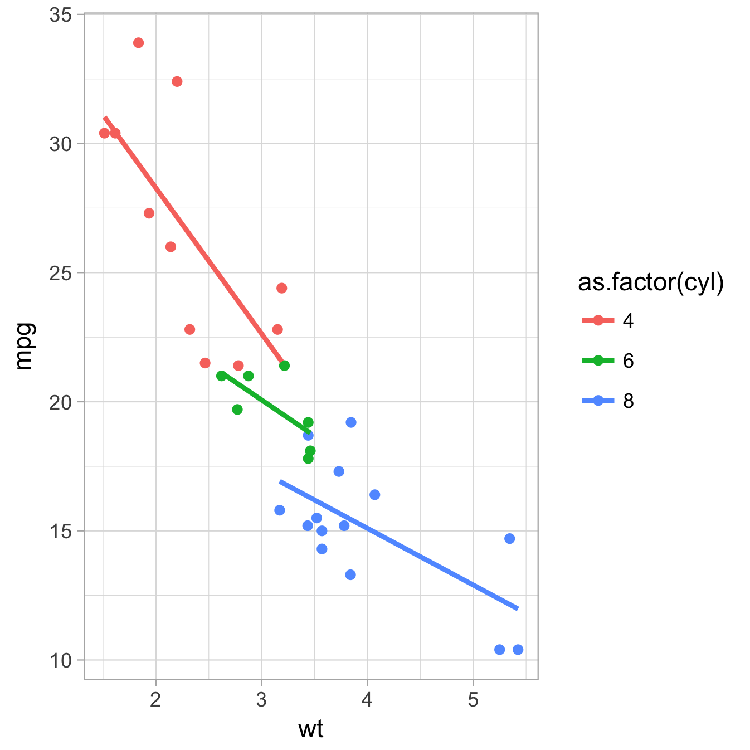
\includegraphics{main_text_files/figure-latex/scatplt-1.pdf}

\textbf{Figure S1}: Scatter plot of XXX. Each point indicates XXXX.

\newpage

\hypertarget{section-2}{%
\section{}\label{section-2}}

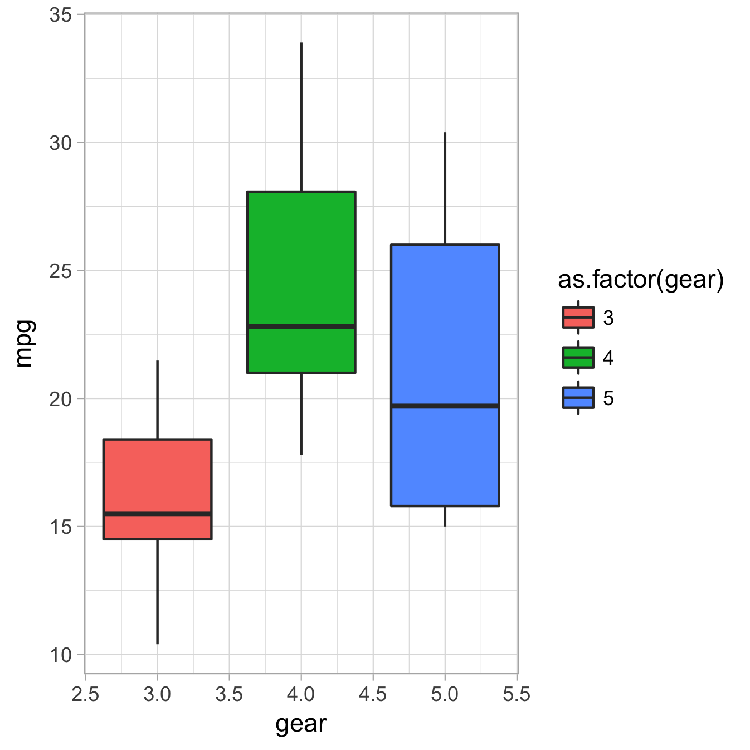
\includegraphics{main_text_files/figure-latex/boxplt-1.pdf}

\textbf{Figure S2}: Boxplot of XXXX.



\newpage
\singlespacing
\end{document}
